\documentclass{article} % For LaTeX2e
\usepackage{cos424,times}
\usepackage{url}
\usepackage{graphicx}
\usepackage{hyperref}
\usepackage{array}
\usepackage{tabu}
\usepackage{cos424,times}
\usepackage{hyperref}
\usepackage{url}
\usepackage{graphicx}
\usepackage{amsmath}
%\usepackage{natbib}
\usepackage{multirow}
\usepackage{bm,bbm}
 \usepackage{amssymb}


\title{Classification of review sentiments}


\author{
Rediet Tilahun Desta\\
Department of Electrical Engineering\\
\texttt{rtilahun@princeton.edu} \\
}

\newcommand{\fix}{\marginpar{FIX}}
\newcommand{\new}{\marginpar{NEW}}

\begin{document}

\maketitle

\begin{abstract}
In this age where we mostly buy products be they clothes or music, we would like to get the opinions of others before making the decision. However going through all reviews can be time consuming. Companies that faciliate this trading process would like to present their customers with a quick and easy way to gauge the overall response to the product; the first step of which will be analyzing the sentiments of each reviews. In this assignment, I attempt to find a good sentiment classifier which would classify reviews as either positive or negative, using a data set of 3000 reviews. I employed Natural Language Processing(NLP) techniques to represent the data as a bag-of-words which were then used to train six types of classifiers.  Multinomial and bernoulli naive bayes classifiers, decision trees and random forest classifiers have high precision and recall, whereas support vector machines have a significant advantage in precision while performing significantly poorly in recall. K-nearest neighbours classifier has relatively good precision but performs poorly on recall.
\end{abstract}

\section{Introduction}
Sentiment analysis used to be a very human task in the past. However in recent years, with the growth of online companies, the need for automated forms of sentiment analysis were found to be of most importance. Online companies like Amazon, Facebook, Twitter and Yelp are increasingly becoming dependent on machine learning algorithms to classify the sentiment of the billions of textual inputs they receive daily. In this assignment, I am interested in learning which type of classifiers perform well in classifying the sentiments of online reviews. Moreover, I want to gain the understanding of why certain classifiers perform well while others less so. 

I evaluate 6 types of classifiers in this report. In the feature extraction process, 


\section{Related Work}
%This is an example for citing an article \cite{zhu2009}.

\section{Methods}

\subsection{One method in detail}

Select one of the methods you chose for application in this assignment and describe in detail the model or objective, the method for inference, and the approach for prediction in future samples. Include a description of the important assumptions relevant for these data and these analytic questions.

\section{Results}

\small
   \centering
   \begin{tabular}{@{}|c|c|c|c|c|c|@{}} % Column formatting, @{} suppresses leading/trailing space 
   \hline

   Classifier & Accu & Prec & Recall & $F_1$ & Time (s) \\ \hline 
      MNB & 0.770 & 0.781 & 0.750 & 0.77 & 0.009 \\
       BNB & 0.773 &  0.788 & 0.747 & 0.767 & 0.045\\
      SVM    &  0.582 & 0.930 & 0.177 & 0.297 & 5.513\\
        DT  &  0.715 & 0.748 & 0.723 & 0.736 & 0.817 \\
      RT &  0.772 & 0.761 & 0.753 & 0.757 & 0.325  \\
      KNN &  0.662 & 0.739 & 0.5 & 0.596 & 2.890 \\
     \hline
   \end{tabular}
   \label{tab:classifiers}

\begin{figure}
\centering
  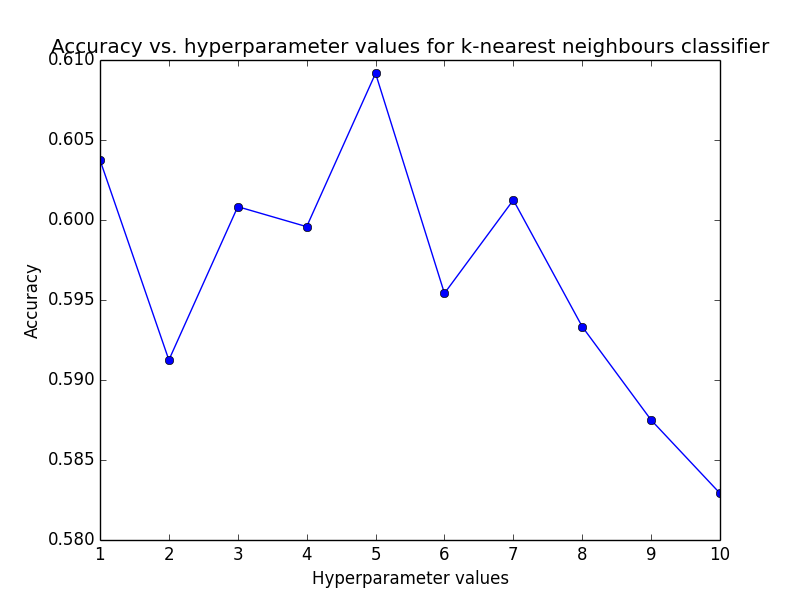
\includegraphics[width=0.5\linewidth]{hyperparameter_fitting_k_nearest.png}
  \caption{A boat.}
  \label{fig:boat1}
\end{figure}

\begin{figure}
\centering
  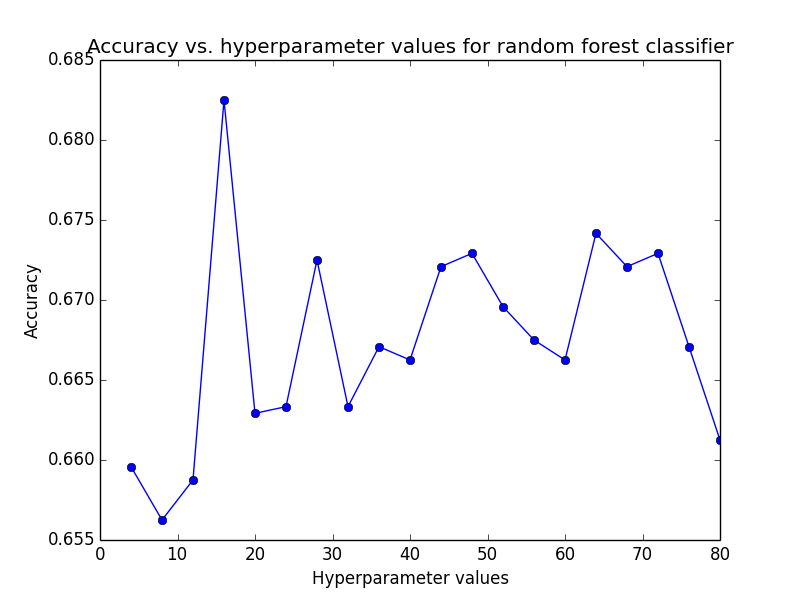
\includegraphics[width=0.5\linewidth]{hyperparameter_fitting_random_forest.png}
  \caption{A boat2.}
  \label{fig:boat2}
\end{figure}


\section{Discussion and Conclusion}

\subsubsection*{Acknowledgments}


\bibliography{ref}
\bibliographystyle{plain}

\end{document}
